\section{System design and implementation}
\label{sec:system-design}

This section describes the architecture and implementation of the developed multi-agent system for code smell detection, prioritization, and refactoring. The system leverages Large Language Models (LLMs) in combination with traditional static analysis tools to provide comprehensive code quality assessment and improvement.

\subsection{System overview}

The developed tool implements a multi-agent architecture where specialized AI agents collaborate to analyze code quality, detect smells, determine refactoring priorities, and execute refactorings. The system integrates:

\begin{itemize}
    \item SonarQube for initial code smell detection using rule-based static analysis
    \item LLM-based agents built using LangGraph framework for intelligent analysis and refactoring
    \item MLflow for experiment tracking, evaluation, and dataset management
    \item Dependency analysis engine that models positive and negative relationships between code smells
    \item Priority calculation system that determines optimal refactoring sequences based on severity and impact
\end{itemize}

The architecture follows a pipeline approach where each agent has a specific responsibility, and agents can communicate context through shared state. This design enables modular development and allows individual agents to be improved independently.

\subsection{Multi-agent architecture}

The system employs six specialized agents working in sequence:

\subsubsection{Agent 1: Code smell detection agent}

The first agent performs static analysis using SonarQube to identify code smells in Java projects. This agent:

\begin{itemize}
    \item Analyzes Java source code at commit-level granularity
    \item Detects the following code smells mapped to SonarQube rules:
    \begin{itemize}
        \item Long Method (java:S138) - Methods exceeding 60 lines of code
        \item Complex Method (java:S1541) - Methods with high cyclomatic complexity
        \item Conditional Complexity (java:S1067) - Deeply nested conditional expressions
        \item Long Parameter List (java:S107) - Methods with more than 7 parameters
        \item God Class (java:S1200) - Classes coupled to too many other classes
        \item Large Class (java:S110) - Classes with excessive lines of code
        \item Duplicated Conditions (java:S1871) - Identical conditional branches
        \item Print Statements (java:S106) - Direct use of System.out/System.err
    \end{itemize}
    \item Returns severity levels (HIGH, MEDIUM, LOW) for each detected smell
    \item Provides line-level location information for each issue
\end{itemize}

The agent is implemented in \texttt{sonarqube/commit\_scan.py} and supports caching of scan results to avoid redundant analysis.

\subsubsection{Agent 2: Test existence verification agent}

The second agent verifies whether unit tests exist for methods containing code smells. This agent:

\begin{itemize}
    \item Detects the build system (Maven or Gradle) in Java projects
    \item Executes the test suite using the detected build system
    \item Analyzes test results to identify which tests passed and which failed
    \item Maps test coverage to specific methods that contain code smells
    \item Reports gaps in test coverage for smelly methods
\end{itemize}

The agent is implemented using LangGraph in \texttt{agents/java\_test/agent.py} and uses LLM-powered tools to detect build configurations and parse test execution output.

\subsubsection{Agent 3: Test generation agent}

\textit{Note: While test generation is an important concern, it is not the primary focus of this research. The emphasis is placed on code smell detection, prioritization, and refactoring. However, the architecture includes a placeholder for this agent to demonstrate the extensibility of the multi-agent system.}

This agent would be responsible for generating tests for methods lacking coverage, but is currently not fully implemented as the research focuses on other aspects of the refactoring workflow.

\subsubsection{Agent 4: Smell prioritization agent}

The fourth agent determines the optimal sequence for refactoring detected smells. This is a critical component that implements the theoretical framework based on smell dependencies and impact analysis.

\paragraph{Theoretical foundation}

The prioritization strategy is based on the work of Markovič and Polášek on code smell dependencies~\cite{markovic2016refaktorovanie}. The approach recognizes that code smells do not exist in isolation - refactoring one smell can affect others through:

\begin{itemize}
    \item Positive dependencies (PZ): Refactoring smell A may simultaneously resolve smell B
    \begin{itemize}
        \item Example: Extracting a Long Method often resolves Duplicated Code, Switch Statements, and Complex Method issues within that method
    \end{itemize}
    \item Negative dependencies (NZ): Refactoring smell A may introduce smell B
    \begin{itemize}
        \item Example: Applying ``Introduce Parameter Object'' to fix Long Parameter List may create a Data Class smell
        \item Example: Splitting a Large Class may introduce Long Method or Data Class smells in the extracted classes
    \end{itemize}
\end{itemize}

\paragraph{Priority calculation algorithm}

The agent calculates a priority score (PZ) for each smell instance:

\begin{equation}
    PZ_i = Severity_i + \sum_{j \in \text{PositiveDeps}(i)} w_{\text{impact}}
\end{equation}

where:
\begin{itemize}
    \item $Severity_i$ is the base severity score: HIGH = 3, MEDIUM = 2, LOW = 1
    \item $\text{PositiveDeps}(i)$ is the set of smells that refactoring smell $i$ would help resolve
    \item $w_{\text{impact}} = 2$ is the weight assigned to each positive impact relationship
\end{itemize}

The refactoring sequence is determined by iteratively selecting the smell with maximum PZ, removing it from the graph, and recalculating scores. This greedy algorithm prioritizes smells that have both high severity and high potential to resolve other smells.

\paragraph{Dependency rules}

The system implements a comprehensive dependency rule base (defined in \texttt{agents/dependency\_analysis/agent.py}):

\begin{itemize}
    \item Long Method / Complex Method / Conditional Complexity
    \begin{itemize}
        \item Positive: May resolve Switch Statement, Feature Envy, Duplicated Code, Divergent Change, Comments, Long Parameter List
        \item Negative: May create Long Method, Long Parameter List
    \end{itemize}

    \item Long Parameter List
    \begin{itemize}
        \item Positive: May resolve Long Parameter List, Data Clumps
        \item Negative: May create Data Class
    \end{itemize}

    \item Large Class / God Class
    \begin{itemize}
        \item Positive: May resolve Data Clumps, Feature Envy, Bad Class Content
        \item Negative: May create Long Method, Data Class, Inappropriate Intimacy, Message Chains
    \end{itemize}

    \item Duplicated Conditions
    \begin{itemize}
        \item Positive: May resolve Divergent Change, Shotgun Surgery
        \item Negative: May create Large Class, Bad Inheritance
    \end{itemize}

    \item Print Statements
    \begin{itemize}
        \item Positive: May resolve Needless Part
        \item Negative: May create Data Class, Lazy Class
    \end{itemize}
\end{itemize}

\paragraph{Visualization}

The agent generates visual representations of the dependency graph (see Figure~\ref{fig:smell-priority-graph}). Nodes represent smell instances, sized according to their PZ score. Green edges indicate positive dependencies (refactoring the source smell helps resolve the target), while red edges indicate negative dependencies (potential risks).

\begin{figure}[h]
    \centering
    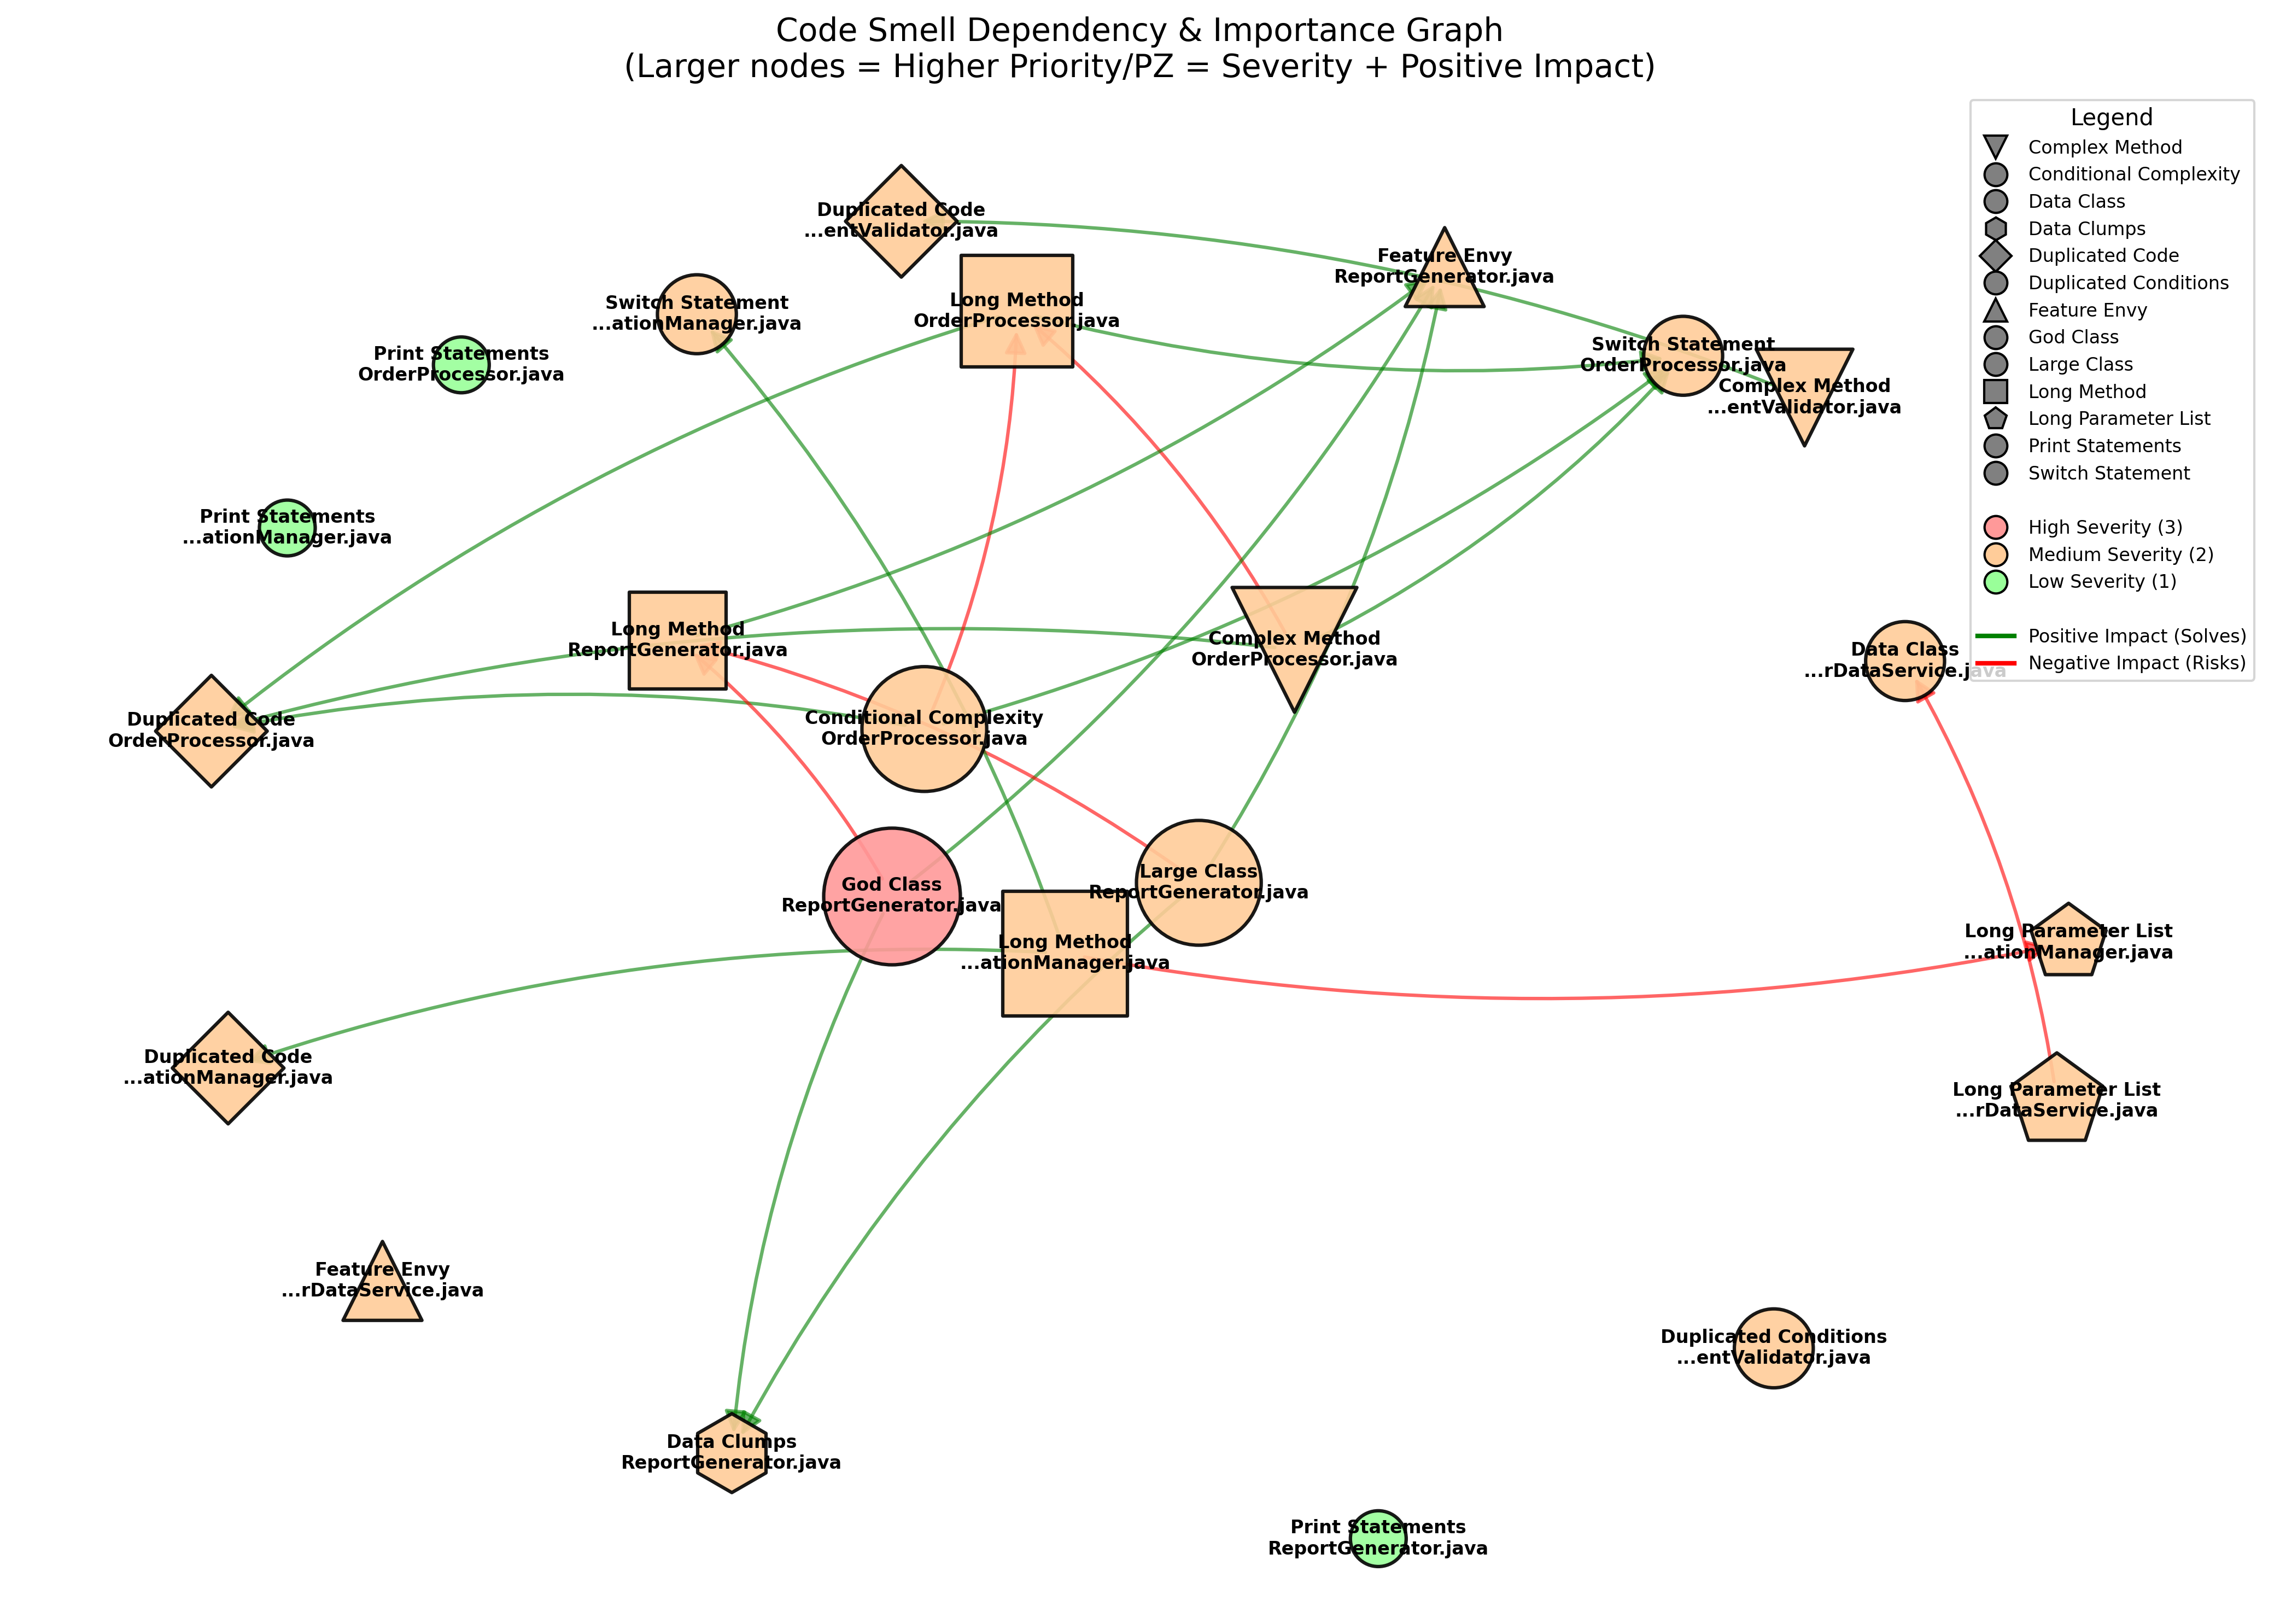
\includegraphics[width=0.9\textwidth]{smell_priority_graph.png}
    \caption{Code smell dependency and priority graph. Node size represents priority score (PZ = Severity + Positive Impact). Green edges show positive dependencies (solving relationships), red edges show negative dependencies (risk of creating new smells).}
    \label{fig:smell-priority-graph}
\end{figure}

The agent also generates file-specific dependency visualizations (see Figure~\ref{fig:smell-deps-orderprocessor}) showing the relationships between smells detected within a single file. These local views help developers understand the immediate impact of refactoring decisions.

\begin{figure}[h]
    \centering
    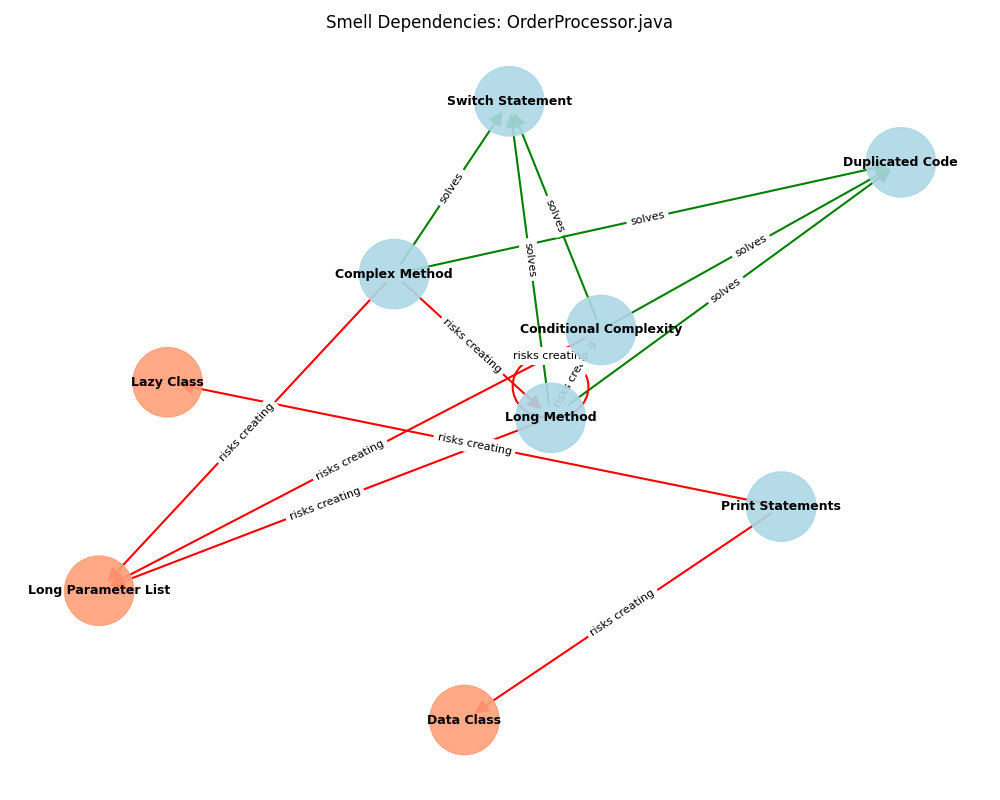
\includegraphics[width=0.8\textwidth]{smell_deps_OrderProcessor.png}
    \caption{Smell dependencies within OrderProcessor.java. This file-level view shows how refactoring one smell (e.g., Long Method) can cascade to resolve multiple related smells (Duplicated Code, Switch Statement, Complex Method).}
    \label{fig:smell-deps-orderprocessor}
\end{figure}

The prioritization agent is implemented in \texttt{scripts/prioritize\_smells.py} and the dependency analysis rules are centralized in \texttt{agents/dependency\_analysis/agent.py}. The workflow for generating dependency visualizations is implemented in \texttt{workflows/smell\_cooccurrence\_workflow.py}.

\subsubsection{Agent 5: Refactoring execution agent}

The fifth agent performs the actual code refactoring based on the prioritized smell sequence. This agent:

\begin{itemize}
    \item Receives the prioritized list of smells from Agent 4
    \item For each smell in sequence, applies appropriate refactoring techniques:
    \begin{itemize}
        \item Long Method: Extract Method refactoring
        \item Large Class/God Class: Extract Class refactoring
        \item Long Parameter List: Introduce Parameter Object
        \item Duplicated Code: Extract Method and remove duplication
        \item Complex Method: Decompose conditional logic
    \end{itemize}
    \item Uses LLM capabilities to understand code context and generate semantically correct refactorings
    \item Preserves code functionality while improving structure
    \item Generates intermediate code versions after each refactoring step
\end{itemize}

The refactoring agent leverages the LangGraph framework and is designed to work with the RefactoringMiner dataset for evaluation purposes.

\subsubsection{Agent 6: Test execution and verification agent}

The sixth agent validates that refactorings preserve program behavior by executing tests. This agent:

\begin{itemize}
    \item Runs the complete test suite after each refactoring
    \item Reports test failures and errors with detailed information
    \item Enables rollback if tests fail after a refactoring
    \item Ensures that code quality improvements do not introduce regressions
\end{itemize}

This agent reuses the test execution capabilities from Agent 2 but focuses on verification rather than coverage analysis.

\subsection{Evaluation framework}

The system uses MLflow for comprehensive experiment tracking and evaluation. This enables:

\begin{itemize}
    \item Dataset management: Creating and versioning datasets from RefactoringMiner data
    \item Experiment tracking: Recording model configurations, parameters, and metrics for each evaluation run
    \item Result comparison: Comparing different approaches (vanilla LLM, RAG-enhanced, hybrid)
    \item Reproducibility: Ensuring experiments can be reproduced with exact configurations
\end{itemize}

The evaluation workflow is documented in \texttt{docs/README\_RMINER.md} and implemented in:
\begin{itemize}
    \item \texttt{scripts/create\_rminer\_dataset.py} - Dataset creation from RefactoringMiner manifest
    \item \texttt{scripts/manage\_datasets.py} - Dataset inspection and management
    \item \texttt{agent\_workflows/rminer\_eval.py} - Evaluation pipeline execution
\end{itemize}

\subsection{Ground truth dataset}

The system is currently evaluated using the RefactoringMiner 2.0 dataset~\cite{tsantalis2022refactoringminer}:

\begin{quote}
Nikolaos Tsantalis, Ameya Ketkar, and Danny Dig. ``RefactoringMiner 2.0.'' \textit{IEEE Transactions on Software Engineering}, vol. 48, no. 3, pp. 930-950, March 2022.
\end{quote}

\paragraph{Dataset properties}
\begin{itemize}
    \item Size: 547 commits from 188 open-source projects
    \item Time range: Commits between June 8, 2015 and August 7, 2015
    \item Content: Real refactorings performed by developers, including:
    \begin{itemize}
        \item Before and after code versions
        \item Refactoring type annotations (Extract Method, Move Method, etc.)
        \item Detailed location information (class, method, line numbers)
        \item Diff hunks showing exact code changes
    \end{itemize}
\end{itemize}

The dataset provides ground truth for evaluating the refactoring mapping agent (Agent 5), which must correctly identify which diff hunks correspond to which refactorings.

\subsection{Test data and smell co-occurrence}

For development and validation purposes, the system includes manually crafted test cases demonstrating smell co-occurrence. These are located in \texttt{tests/test\_data/smell\_cooccurrence/} and include:

\begin{itemize}
    \item OrderProcessor.java: Demonstrates positive dependencies in the ``bad size'' category (Long Method, Complex Method, Duplicated Code, Switch Statement)
    \item CustomerDataService.java: Demonstrates negative dependencies (Long Parameter List vs. Data Class trade-off)
    \item ReportGenerator.java: Demonstrates God Class with multiple interconnected smells
    \item PaymentValidator.java: Demonstrates duplicated conditions and their dependencies
    \item ConfigurationManager.java: Demonstrates complex interplay of multiple smells
\end{itemize}

Each test file is annotated in \texttt{smells\_manifest.json} with the smells present, their locations, severities, and descriptions. This enables:
\begin{itemize}
    \item Testing the smell detection agent's accuracy
    \item Validating dependency analysis rules
    \item Demonstrating the prioritization algorithm with known smell relationships
    \item Visualizing how smells co-occur in realistic code patterns
\end{itemize}

\subsection{Code metrics and refactoring impact analysis}

After each refactoring, the system evaluates code quality improvements using standard object-oriented metrics:

\begin{itemize}
    \item WMC (Weighted Methods per Class): Sum of cyclomatic complexities of all methods in a class
    \item CBO (Coupling Between Objects): Number of classes to which a class is coupled
    \item RFC (Response For a Class): Number of methods that can potentially be executed in response to a message received by an object
    \item LCOM (Lack of Cohesion of Methods): Measures how methods and attributes are related
\end{itemize}

These metrics validate that refactorings achieve their intended goals. For example:
\begin{itemize}
    \item Extracting a Long Method should reduce WMC
    \item Splitting a God Class should reduce CBO and RFC
    \item Resolving Feature Envy should improve LCOM
\end{itemize}

The system also tracks how positive and negative dependencies manifest in practice:

\paragraph{Positive dependencies validation}
After refactoring a smell, the system checks whether predicted positive dependencies were realized:
\begin{itemize}
    \item If Long Method is refactored, does Duplicated Code decrease?
    \item If Large Class is split, does Feature Envy reduce?
\end{itemize}

\paragraph{Negative dependencies monitoring}
The system monitors whether refactorings introduce predicted negative dependencies:
\begin{itemize}
    \item After applying ``Introduce Parameter Object'', is a Data Class created?
    \item After splitting a Large Class, do Long Methods appear in extracted classes?
\end{itemize}

This feedback loop enables the system to learn which dependency rules are accurate in practice and adjust priorities accordingly.

\subsection{Implementation technologies}

The system is implemented using:

\begin{itemize}
    \item Python 3.11+: Core implementation language
    \item LangGraph: Framework for building multi-agent workflows with state management
    \item LangChain: LLM orchestration and tool integration
    \item LiteLLM: Unified interface for multiple LLM providers (OpenAI, Anthropic, Google)
    \item MLflow: Experiment tracking and dataset management
    \item SonarQube: Static code analysis engine
    \item NetworkX: Graph analysis and dependency modeling
    \item Matplotlib: Visualization of dependency graphs
    \item Pydantic: Data validation and structured outputs from LLMs
\end{itemize}

The modular architecture allows different LLM models to be used for different agents based on task complexity:
\begin{itemize}
    \item GPT-4o-mini: Default model for most agents (cost-effective)
    \item GPT-4o: For complex refactoring tasks requiring deeper reasoning
    \item Claude Sonnet: Alternative for specific agent implementations
    \item Gemini 2.5: Used in RAG experiments for code understanding
\end{itemize}

\subsection{Workflow execution}

A complete analysis and refactoring workflow proceeds as follows:

\begin{enumerate}
    \item Initial scan: Agent 1 analyzes a commit using SonarQube and identifies code smells
    \item Test verification: Agent 2 checks test coverage for affected methods
    \item Dependency analysis: Agent 4 analyzes smell dependencies and calculates PZ scores
    \item Priority determination: Agent 4 generates refactoring sequence based on maximum PZ strategy
    \item Visualization: System generates dependency graphs and priority visualizations
    \item Refactoring execution: Agent 5 applies refactorings in priority order
    \item Verification: Agent 6 runs tests after each refactoring to ensure correctness
    \item Metrics evaluation: System calculates code quality metrics before and after
    \item Result logging: MLflow records all steps, decisions, and outcomes
\end{enumerate}

This workflow ensures that refactorings are applied systematically, with continuous validation and detailed tracking for research analysis.
